\documentclass[twoside]{article}

\usepackage{ustj}
\usepackage{cancel}
\usepackage{pdflscape}

\usepackage{tikz}
\newcommand{\bit}[1]{%
  \tikz[baseline=(char.base)]{%
    \node[shape=rectangle, draw, rounded corners=1pt, inner sep=1pt, minimum width=6pt, minimum height=6pt] (char) {#1};
  }%
}
% support vertex
\newcommand{\vertex}[1]{%
  \tikz[baseline=(char.base)]{%
    \node[shape=circle, draw, inner sep=1pt, minimum size=6pt] (char) {#1};
  }%
}

\setcounter{tocdepth}{2}

\addbibresource{mss.bib}

\newcommand{\authorname}{N. E. Davis \patp{lagrev-nocfep},* \& Sam Parker \patp{borlug-walryd}†}
\newcommand{\affiliation}{* ZeroAttest, Groundwire Foundation,\\Urbit Development Institute \\ † —}

%  Make first page footer:
\fancypagestyle{firststyle}{%
\fancyhf{}% Clear header/footer
\fancyhead{}
\fancyfoot[L]{{\footnotesize
              %% We toggle between these:
              Manuscript submitted for review.\\
              % {\it Urbit Systems Technical Journal} II:2 (2025):  1–46. \\
              % ~ \\
              % Address author correspondence to \authorpatp.
              }}
}
%  Arrange subsequent pages:
\fancyhf{}
\fancyhead[LE]{{\urbitfont Urbit Systems Technical Journal}}
\fancyhead[RO]{Noun Graph Encoding}
\fancyfoot[LE,RO]{\thepage}

%%MANUSCRIPT
\title{Noun Graph Encoding}
\author{N. E. Davis \patp{lagrev-nocfep},* \\ \& Sam Parker \patp{borlug-walryd}† \\ \affiliation}
\date{}

\begin{document}

\maketitle
\thispagestyle{firststyle}

\begin{abstract}
Serialization schemes such as \texttt{+jam} encode a noun as a linear byte array in which shared structure is expressed by positional back-reference.  A complementary strategy is to encode the noun as an explicit directed acyclic graph whose nodes are its distinct subnouns.  Where \texttt{+jam} is a communications format, this graph form is a store format, affording total deduplication, random access to subtrees, incremental update, and content-addressed identity.  We describe the shared core of such an encoding and organize its variants along a small set of design axes.  We show that two coherent configurations bracket the design space:  a local, selectively grained \texttt{\$silo} after the manner of \patp{sorreg-namtyv}'s ``grains'' proposal, and a globally content-\linebreak addressed store \texttt{\$bulk}.  Globally recomputable identity requires canonical graining, which forecloses the granularity control on which the local design depends.
\end{abstract}

% We will adjust page numbering in final editing.
\pagenumbering{arabic}
\setcounter{page}{1}

\tableofcontents

\section{Introduction}

A noun is an abstract binary tree, and a serialization scheme is a way of writing that tree down.\footnote{An earlier companion article on noun serialization described \texttt{+jam} (\patp{ticlys-monlun} \& \patp{lagrev-nocfep}, ``Noun Serialization,'' \emph{Urbit Systems Technical Journal} volume 3 issue 1, pp.~83--101).}  The conventional scheme, \texttt{+jam} serialization, encodes a noun as a single atom:  a linear bitstream in which the tree is walked in depth-first order and shared subtrees are elided by positional back-reference---a repeated subnoun is written once and thereafter named by the bit offset at which its encoding began.  This design serves well as an archive:  a self-contained, one-shot representation to be written to a file, sent over a wire, or hashed as a unit.  It is a poor design for a store.  A store must answer questions that an archive need not:  it must deduplicate structure that recurs across many nouns and not merely within one; it must permit a subnoun to be fetched without materializing the whole;\footnote{But see the \texttt{+sip} lazy jam cursor proposal (\urbitpr{7385}).} it must accommodate the incremental replacement of small parts of large evolving structures without rewriting the whole; and it may need to name a subnoun by an identity that a second party can independently recompute.  Positional back-reference serves none of these:  an offset is meaningful only within the single stream that defines it, is invalidated by any edit that shifts it, and says nothing about the noun it points to.

The natural store representation is the one the runtime already keeps in memory.  Vere and NockVM do not store the $1.66 \times 10^{21}$ nouns of a running Arvo as trees;\footnote{A computation due to \patp{dozreg-toplud}.} they store a reference-counted directed acyclic graph in which each distinct subnoun is a single, shared, pointer-identified object, and structural equality is short-circuited to pointer equality.\footnote{See \patp{rovyns-ricfer} and \patp{wicdev-wisryt}, ``A Solution to Static vs. Dynamic Linking,'' \emph{Urbit Systems Technical Journal} volume 1 issue 1, pp.~75--82.}  This article asks what it means to write such an object; to wit, to serialize the sharing graph itself, rather than a tree that happens to share.

\section{Directed Graph Encoding}

If references to subnouns are permitted in a serialization scheme, then it is possible to conceive of mapping a binary tree to a directed graph representation.  Each unique subtree is represented as a node in the directed graph, and edges point to child nodes.  This allows for a different efficient representation of shared subtrees (Figure~\ref{fig:binary-tree-dag}).  (A noun and any representation of it are still acyclic, so the directed graph is a directed acyclic graph, or \textsc{dag}.)  In fact, the idea of using this for the memoization of subject--formula pairs has long been considered.

A directed graph encoding has been independently proposed twice, once by Curtis Yarvin \patp{sorreg-namtyv} TODO incidental to the ``grains'' proposal\footnote{Circulated as \texttt{grains.txt}, this document dates to \textasciitilde 2019.3.6.  At the time of writing, a copy was available at \url{https://gist.github.com/Fang-/60b125e6e9ee0c7eec74d066b12210ef}.} as a \lstinline[style=inlinecode]{$silo} encoding and again by Sam Parker \patp{borlug-walryd} as the \lstinline[style=inlinecode]{$bulk} encoding.  The two proposals differ in ambition, and the bulk of this article is devoted to showing that the difference is not incidental but structural (Section~\ref{sec:axes}).

\begin{figure}[htp]
  \centering
    \centering
    \begin{subfigure}{\textwidth}
      \centering
      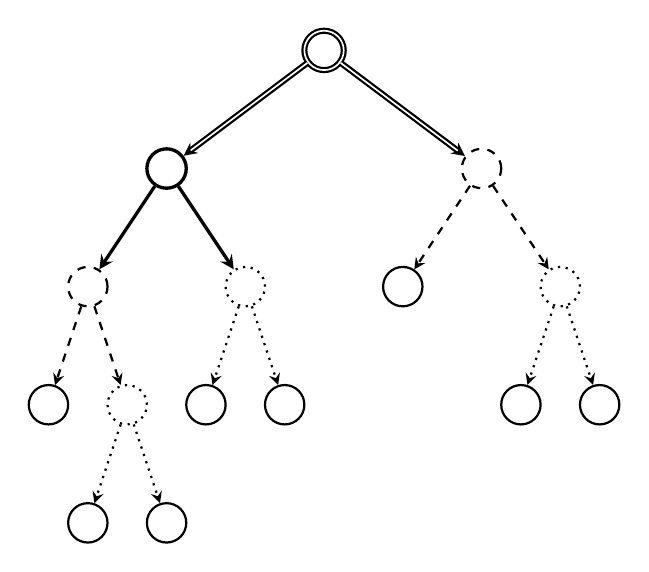
\begin{tikzpicture}[
          level 1/.style={sibling distance=40mm, line width=1pt},
          level 2/.style={sibling distance=20mm, line width=1pt},
          level 3/.style={sibling distance=10mm, line width=1pt},
          level 4/.style={sibling distance=10mm, line width=1pt},
          every node/.style={circle, draw, line width=1pt, minimum size=1.2em},
          every node/.style={circle, draw, minimum size=0.5cm, thick},
          >=stealth
        ]
        % 1
        \node[double, thick] {}
          child[edge from parent/.style={draw, ->, double, thick}] { 
            %2
            node[very thick] {}
            child[edge from parent/.style={draw, ->, very thick}] { 
              %4
              node[dashed, thick] {}
              child[edge from parent/.style={draw, ->, dashed, thick}] { 
                %8
                node {} }
              child[edge from parent/.style={draw, ->, dashed, thick}] { 
                %9
                node[dotted, thick] {}
                child[edge from parent/.style={draw, ->, dotted, thick}] { 
                  %18
                  node[solid, thick] {} }
                child[edge from parent/.style={draw, ->, dotted, thick}] { 
                  %19
                  node[solid, thick] {} }
              }
            }
            child[edge from parent/.style={draw, ->, very thick}] { 
              %5
              node[dotted, thick] {}
              child[edge from parent/.style={draw, ->, dotted, thick}] { 
                %10
                node {} }
              child[edge from parent/.style={draw, ->, dotted, thick}] { 
                %11
                node {} }
            }
          }
          child[edge from parent/.style={draw, ->, double, thick}] { 
            %3
            node[dashed, thick] {}
            child[edge from parent/.style={draw, ->, dashed, thick}] { 
              %6
              node {} }
            child[edge from parent/.style={draw, ->, dashed, thick}] { 
              %7
              node[dotted, thick] {}
              child[edge from parent/.style={draw, ->, dotted, thick}] { 
                %14
                node[solid, thick] {} }
              child[edge from parent/.style={draw, ->, dotted, thick}] { 
                %15
                node[solid, thick] {} }
            }
          };
      \end{tikzpicture}
    \end{subfigure}
    \\
    \begin{subfigure}{\textwidth}
      \centering
      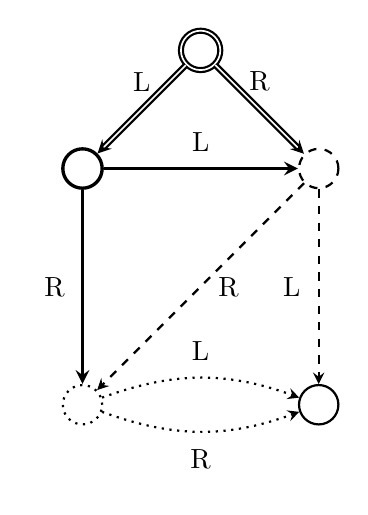
\begin{tikzpicture}[
        node distance=3cm,
        every node/.style={circle, draw, minimum size=0.5cm, thick},
        vertex/.style={circle, draw, minimum size=0.5cm, thick},
        >=stealth
      ]
        % Define the four nodes in a square
        \node[vertex, double, thick] (Root) at (1.5,4.5) {};
        \node[vertex, very thick] (A) at (0,3) {};
        \node[vertex, dashed, thick] (B) at (3,3) {};
        \node[vertex, dotted, thick] (C) at (0,0) {};
        \node[vertex, thick] (D) at (3,0) {};

        \draw[->, double, thick] (Root) -- node[above, draw=none] {L} (A);
        \draw[->, double, thick] (Root) -- node[above, draw=none] {R} (B);

        \draw[->, very thick] (A) -- node[above, draw=none] {L} (B);
        \draw[->, very thick] (A) -- node[left, draw=none] {R} (C);

        \draw[->, dashed, thick] (B) -- node[right, draw=none] {R} (C);
        \draw[->, dashed, thick] (B) -- node[left, draw=none] {L} (D);

        \draw[->, dotted, thick, bend left=20] (C) to node[above, draw=none] {L} (D);
        \draw[->, dotted, thick, bend right=20] (C) to node[below, draw=none] {R} (D);
      \end{tikzpicture}
    \end{subfigure}
  \caption{The noun \texttt{[[a a a] a a] [a a a]} as a binary tree and its metadata labeling in a directed graph representation.}
  \label{fig:binary-tree-dag}
\end{figure}

\subsection{The Shared Core}

Several distinct encodings answer to the description ``directed graph,'' and they differ in load-bearing ways (Section~\ref{sec:axes}).  They share a common skeleton, however, which we fix first and vary afterward (Figure~\ref{fig:binary-tree-dag}).

A noun is mapped to a set of \emph{nodes}, one per distinct subnoun under structural equality.  A node is either an \emph{atom node}, carrying an atomic value, or a \emph{cell node}, carrying an ordered pair of \emph{references} to its head and tail nodes.  Exactly one node---the whole noun---is the \emph{root}.  Because a node exists once per distinct subnoun, deduplication is total:  a subnoun that occurs a thousand times is one node referenced a thousand times, in contrast to \texttt{+jam}, whose back-referencing is gated on a size heuristic and elides a repeat only when the reference is shorter than the subtree it replaces.

Three commitments make the skeleton concrete and, together, make decoding safe:

\begin{itemize}
\item  \textbf{Leaves reuse \texttt{+mat}.}  An atom node encodes its value with the \texttt{+mat} codec.\footnote{There is no reason to devise a second length-encoding for atoms, and reusing \texttt{+mat} keeps the leaf-level output bit-for-bit comparable with \texttt{+jam}.}
\item  \textbf{Nodes are emitted in topological order.}  Children are written before parents, so the root is written last.  A single forward pass suffices to reconstruct:  when a cell node is read, the nodes it references have already been built.
\item  \textbf{References point only backward.}  A reference names an already-emitted node.  Consequently a reference cycle is unrepresentable, and the decoder rejects any reference to an as-yet-undefined node.  Since a noun is always finite and acyclic, this costs no expressiveness, but it does purchase a guarantee that a hostile or corrupt byte array cannot drive the decoder into a loop.\footnote{This is the graph-encoding counterpart of the leading-zero and length-delimiter discipline that makes \texttt{+cue} unambiguous.}
\end{itemize}

\noindent
The skeleton leaves one thing deliberately abstract:  what a reference \emph{is}.  A reference may be a positional index into the emitted sequence, a strong hash of the referent, or a canonical content hash.  The whole design turns on this axis (Section~\ref{sec:axes}).  For a concrete worked example we take the simplest choice, the positional index; the others will substitute a different reference codec into the identical skeleton.

\subsection{A Worked Example}

Consider the noun of Figure~\ref{fig:binary-tree-dag}, \texttt{[[a a a] a a] [a a a]}.  Its distinct subnouns, in topological (children-first) order, are five:

\begin{table}[ht]
\centering
\caption{Node table for \texttt{[[a a a] a a] [a a a]}.  Indices are assigned in emission order; every reference is to a strictly smaller index, and the root is last.  Labels correspond to the vertices of Figure~\ref{fig:binary-tree-dag}.}
\label{tab:bulk-nodes}
\begin{tabular}{ r l l l }
  \textbf{Index} & \textbf{Kind} & \textbf{Contents} & \textbf{Fig.} \\
  \hline
  \texttt{0} & atom & \texttt{a}                    & D \\
  \texttt{1} & cell & \texttt{(0,\,0)} \quad(\texttt{[a a]})       & C \\
  \texttt{2} & cell & \texttt{(0,\,1)} \quad(\texttt{[a a a]})     & B \\
  \texttt{3} & cell & \texttt{(2,\,1)} \quad(\texttt{[[a a a] a a]}) & A \\
  \texttt{4} & cell & \texttt{(3,\,2)} \quad(\textrm{root})        & Root \\
\end{tabular}
\end{table}

\noindent
Encoding each node as a type bit---\texttt{0} for atom, \texttt{1} for cell---followed by the \texttt{+mat} encoding of its value (for atoms) or of each reference index (for cells) yields the following stream, one line per node, with \texttt{.} delimiting fields:

\begin{lstlisting}[style=listingblock]
node 0:  0 . (mat a)
node 1:  1 . 1 . 1
node 2:  1 . 1 . 110
node 3:  1 . 100100 . 110
node 4:  1 . 110100 . 100100
\end{lstlisting}

\noindent
Taking \texttt{a} to be the byte \texttt{0x61} (so \texttt{(mat a)} is 13 bits after the type bit) the whole noun encodes in 45 bits.  The economy of the store form is seen by wrapping the noun in a cell with itself, \texttt{[N N]}:  this adds a single cell node, \texttt{(4,\,4)}, and 15 bits---not a second copy of the 45.  A reference to an arbitrarily large structure costs one node.

\paragraph*{Directed Graph Serialization Algorithm}
\begin{itemize}
\item  \textbf{Encode.}  Maintain a map from subnoun to assigned index.  Visit the noun; for each subnoun not already mapped, recursively assign its children first, then emit its node---\texttt{0} and \texttt{(mat value)} for an atom, or \texttt{1} and the \texttt{+mat}-encoded head and tail references for a cell---and record its index.  The root is emitted last.
\item  \textbf{Decode.}  Read nodes in order into an indexed table.  For a \texttt{0} tag, \texttt{+rub} the value and append an atom.  For a \texttt{1} tag, \texttt{+rub} two references; if either names an index not yet present, reject the input as non-topological.  Otherwise append the cell of the referenced nodes.  The last node built is the root.
\end{itemize}

\noindent
A reference implementation is given in the appendix and is bit-compatible with the \texttt{+mat}/\texttt{+rub} of the companion article.

\section{The Design Axes}
\label{sec:axes}

The skeleton of Section~2 is not a single format but a family, and the members differ enough in their properties that naming one ``the'' graph encoding obscures the choice being made.  We organize the family along the axes of Table~\ref{tab:axes}.  Several axes are fixed by the shared core; the remainder are free, and the free axes are not independent.

\begin{table}[ht]
\centering
\caption{Design axes for a directed-graph noun encoding.  The upper block is fixed by the shared core; the lower block is free.  The two rightmost columns name the coherent configurations of Sections~\ref{sec:silo} and~\ref{sec:cas}.}
\label{tab:axes}
\begin{tabular}{ l l l }
  \textbf{Axis} & \textbf{A:\ local silo} & \textbf{B:\ canonical store} \\
  \hline
  Leaf codec        & \multicolumn{2}{c}{\texttt{+mat} (shared)} \\
  Reference order   & \multicolumn{2}{c}{topological, children-first (shared)} \\
  Cycle handling    & \multicolumn{2}{c}{unrepresentable by construction (shared)} \\
  \hline
  Node identity     & local strong hash & canonical injective hash \\
  Graining policy   & selective, hinted & canonical (every cell) \\
  Sharing / export  & pseudocapability  & plain content address \\
  Reclamation       & reference counting & mark-and-sweep \textsc{gc} \\
  Canonical form    & no                & yes \\
  On-disk alignment & tunable           & tunable \\
\end{tabular}
\end{table}

The decisive axis is \emph{node identity}, and its decisive interaction is with \emph{graining policy}.  \emph{Graining} is the choice of which subnouns are promoted to nodes.  The shared core, as presented, grains every distinct subnoun; but a store need not, and for good reason ought not.  Registering every cell of a large structure as an independently addressed node imposes per-node overhead---an identity, a table entry, a reference count---that for small or short-lived subnouns dwarfs the structure it describes.  \patp{sorreg-namtyv}'s proposal accordingly makes graining \emph{selective}:  a subnoun becomes a grain only when hinted, at ``natural boundaries of large-scale objects,'' and unregistered subnouns (``granules'') are simply inlined into the enclosing grain as ordinary tree structure.  Too fine a grain wastes space on overhead; too coarse a grain wastes it on copying.  Graining is thus a tuning knob, and its existence as a knob is the whole economic argument for the local design.

But a tunable node set is incompatible with a globally meaningful identity, and this is the crux of the entire matter.

\paragraph*{Proposition.}
\textit{A node identity that any party can recompute from the noun alone---a content address in the global sense---requires that the node set be a function of the noun alone; that is, it requires canonical graining.}

\paragraph*{Proof.}
The identity of a cell node is a function of the identities of its children, and so, transitively, the identity of the root is a function of the entire node set beneath it.  If graining is selective, the node set is a function of the graining policy as well as of the noun:  two parties applying different policies to structurally equal nouns register different sets of subnouns, present the root with different children, and therefore compute different root identities.  The root identity is then not a function of the noun alone and is not recomputable by a party who does not share the policy.  Contrapositively, for the root identity to be recomputable from the noun alone, the node set must be determined by the noun alone, which is canonical graining. \hfill$\square$

\paragraph*{Corollary.}
\textit{No configuration offers both globally recomputable identity and tunable granularity.  A store must choose:  the granularity knob of the local design, or the recomputable identity of the global one.}

\bigskip
\noindent
This is why \patp{sorreg-namtyv}, whose stated aims were local deduplication and cheap peer-to-peer sharing, explicitly declined global content-addressability and shared grains instead by \emph{pseudocapability}---a grain's hash encrypted under a per-neighbor secret, which grants recomputable identity to chosen counterparties without conceding it to the world.  It is equally why a store intended as a substrate for shared or verifiable state---the setting of content-addressed object stores and of on-chain commitments---must pay for canonical graining and cannot recover the knob.  The two configurations named in Table~\ref{tab:axes} are therefore not two points on a continuum but the two corners the proposition permits.  Sections~\ref{sec:silo} and~\ref{sec:cas} develop each in turn.

\section{Configuration A:\ The Local Silo}
\label{sec:silo}

TODO --- shop/silo segmentation, the grain bit, reference counting (grain-to-grain counted, shop-to-silo uncounted), hint-driven graining, a cheap strong hash, deep memoization as a map beside the dedup set, and pseudocapability export.

\section{Configuration B:\ The Canonical Content-Addressed Store}
\label{sec:cas}

TODO --- canonical graining (grain every distinct cell, coinciding with the hash-consed Merkle \textsc{dag}), the injective domain-separated noun hash, plain content addresses, garbage collection, and the relationship to Git object stores, \textsc{ipfs}, and the \textsc{zk}\textsc{vm} noun commitment.

\tombstone

\selectlanguage{USenglish}
% \printbibliography

\newpage
\section*{Appendix:\ Python Reference}
\addcontentsline{toc}{section}{Appendix:\ Python Reference}

The following is a reference implementation of the shared-core encoding in the positional-index configuration.  The \texttt{mat} and \texttt{rub} routines are those of the companion article and are reproduced for self-containment.

\begin{lstlisting}[style=listingcode_python]
from dataclasses import dataclass

@dataclass(frozen=True)
class Cell:
    head: object
    tail: object

def deep(n): return isinstance(n, Cell)

def mat(bits, i):
    if i == 0:
        bits.append(1); return
    a = i.bit_length(); b = a.bit_length()
    above, below = b + 1, b - 1
    for k in range(above): bits.append(((1 << b) >> k) & 1)
    for k in range(below): bits.append(((a & ((1 << below) - 1)) >> k) & 1)
    for k in range(a):     bits.append((i >> k) & 1)

def rub(bits, pos):
    z = 0
    while bits[pos] == 0: z += 1; pos += 1
    pos += 1
    if z == 0: return 0, pos
    below = z - 1
    low = 0
    for k in range(below): low |= bits[pos] << k; pos += 1
    a = (1 << below) | low
    val = 0
    for k in range(a): val |= bits[pos] << k; pos += 1
    return val, pos

def encode(noun):
    order, index = [], {}
    def visit(n):
        if n in index: return index[n]
        node = ('cell', visit(n.head), visit(n.tail)) if deep(n) else ('atom', n)
        i = len(order); order.append(node); index[n] = i
        return i
    visit(noun)
    bits = []
    for node in order:
        if node[0] == 'atom':
            bits.append(0); mat(bits, node[1])
        else:
            bits.append(1); mat(bits, node[1]); mat(bits, node[2])
    return bits

def decode(bits):
    pos, table = 0, []
    while pos < len(bits):
        tag = bits[pos]; pos += 1
        if tag == 0:
            v, pos = rub(bits, pos); table.append(v)
        else:
            h, pos = rub(bits, pos); t, pos = rub(bits, pos)
            if h >= len(table) or t >= len(table):
                raise ValueError("non-topological reference")
            table.append(Cell(table[h], table[t]))
    return table[-1]
\end{lstlisting}

\end{document}
